%**************************************************************************************
% License:
% CC BY-NC-SA 4.0 (http://creativecommons.org/licenses/by-nc-sa/4.0/)
%**************************************************************************************

\documentclass[notes]{beamer}

\mode<presentation> {

\usetheme{Madrid}

% Burnt orange
\definecolor{burntorange}{rgb}{0.8, 0.33, 0.0}
\colorlet{beamer@blendedblue}{burntorange}
% Pale yellow
\definecolor{paleyellow}{rgb}{1.0, 1.0, 0.953}
\setbeamercolor{background canvas}{bg=paleyellow}
% Secondary and tertiary palette
\setbeamercolor*{palette secondary}{use=structure,fg=white,bg=burntorange!80!black}
\setbeamercolor*{palette tertiary}{use=structure,fg=white,bg=burntorange!60!black}

% To remove the navigation symbols from the bottom of all slides uncomment this line
%\setbeamertemplate{navigation symbols}{}
}

\usepackage{amsmath}
\DeclareMathOperator*{\argmin}{arg\,min}
\DeclareMathOperator*{\argmax}{arg\,max}
\usepackage{bm}
\usepackage{booktabs} % Allows the use of \toprule, \midrule and \bottomrule in tables
\usepackage{breqn}
\usepackage{cleveref}
\usepackage{graphicx} % for figures
\usepackage[labelsep=space,tableposition=top]{caption}
\renewcommand{\figurename}{Fig.} 
\usepackage{caption,subcaption}% http://ctan.org/pkg/{caption,subcaption}
\usepackage{xcolor}
\usepackage{listings} % For code listings

% Python style for listings
\lstdefinestyle{pythonstyle}{
    language=Python,
    basicstyle=\ttfamily\small,
    otherkeywords={self},             
    keywordstyle=\color{blue},
    emph={torch, nn, optim},      
    emphstyle=\color{red},    
    stringstyle=\color{orange},
    commentstyle=\color{green},
    showstringspaces=false,
    frame=tb,
    tabsize=4
}

\AtBeginSection[]{
	\begin{frame}{Outline}
		\tableofcontents[
		currentsection,      % highlight the current section
		hideallsubsections   % show only section titles
		]
	\end{frame}
}

%----------------------------------------------------------------------------------------
%	TITLE PAGE
%----------------------------------------------------------------------------------------
\title[Automatic Differentiation]{Automatic Differentiation: The Engine of Machine Learning} 
\author{Krishna Kumar} % name
\institute[UT Austin] % institution 
{
University of Texas at Austin \\
\medskip
\textit{
  \url{krishnak@utexas.edu}} % Your email address
}
\date{} % Date, can be changed to a custom date

\begin{document}

\begin{frame}
\titlepage % title page as the first slide
\end{frame}

\begin{frame}
 \frametitle{Overview}
 \tableofcontents
\end{frame}

\begin{frame}
\frametitle{Why Do We Need Derivatives?}

Derivatives are the mathematical engine driving modern scientific computing.

\begin{itemize}
    \item \textbf{Optimization:} Finding the minimum of a loss function.
    \item \textbf{Machine Learning:} Training neural networks via gradient descent.
    \item \textbf{Inverse Problems:} Estimating parameters from data (e.g., geophysics).
    \item \textbf{Scientific Machine Learning:} Differentiable simulators, PINNs, Neural ODEs.
\end{itemize}

\vspace{1cm}

\textbf{Challenge:} How do we compute derivatives of complex, computer-implemented functions efficiently and accurately?

\end{frame}

%------------------------------------------------
\begin{frame}
\frametitle{The Four Modes of Differentiation}

Traditionally, we have had three approaches, each with fundamental flaws.

\begin{figure}[ht]
	\centering
	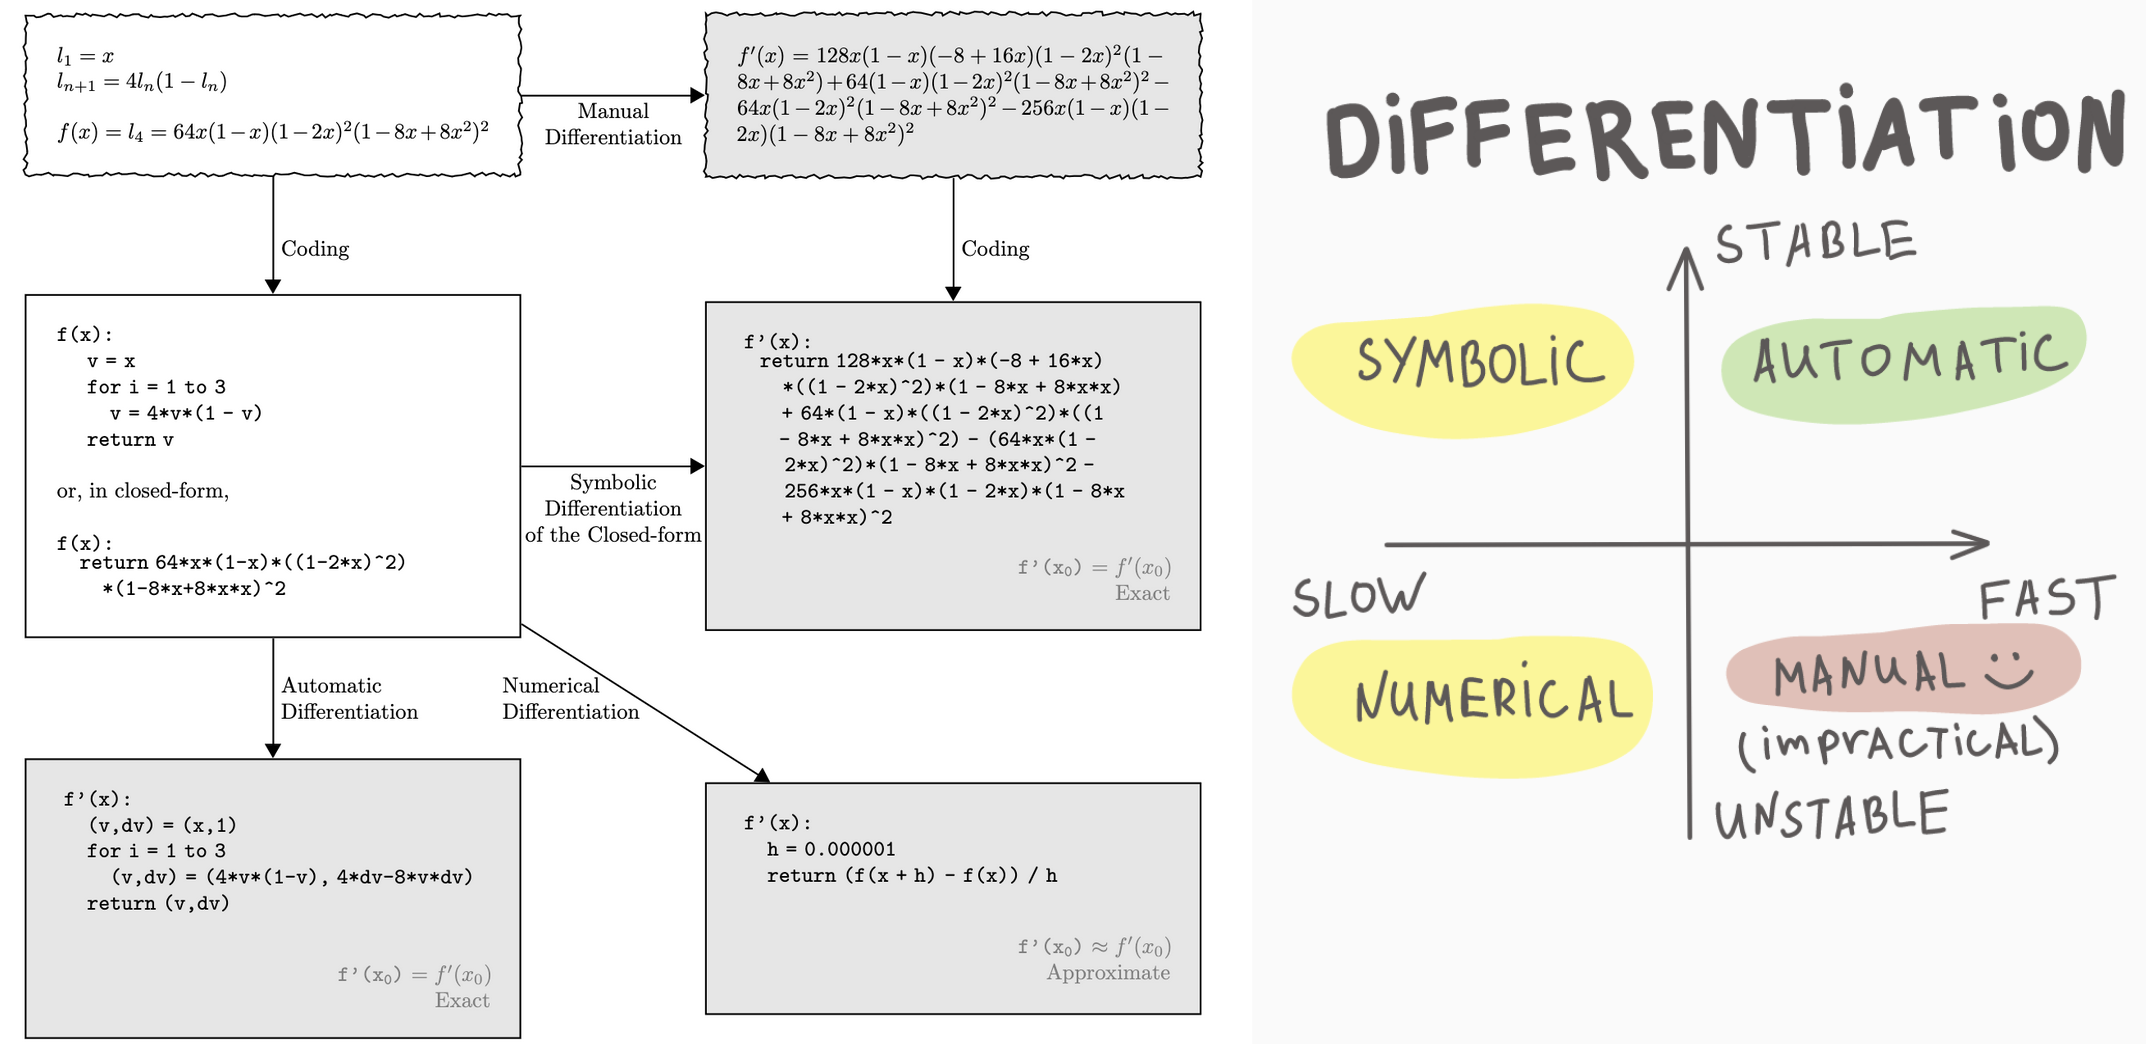
\includegraphics[width=0.9\textwidth]{figs/differentiation.png}
\end{figure}

\begin{itemize}
    \item \textbf{Manual:} Exact, but slow, error-prone, and not scalable.
    \item \textbf{Symbolic:} Exact, but suffers from "expression swell" and is computationally expensive.
    \item \textbf{Numerical (Finite Diff.):} Simple, but suffers from accuracy issues and high computational cost.
\end{itemize}

\textbf{A fourth mode is needed:} Automatic Differentiation (AD).

\end{frame}

%----------------------------------------------------------------------------------------
\begin{frame}
\frametitle{Functions are Computational Graphs}

Every function implemented as a computer program can be decomposed into a sequence of elementary operations.

Consider the function: $y = x_1^2 + x_2$

%\begin{lstlisting}[style=pythonstyle]
%def f(x1, x2):
%    y = x1**2 + x2
%    return y
%\end{lstlisting}

This can be viewed as a computational graph where each operation is a node.

\begin{figure}[ht]
	\centering
	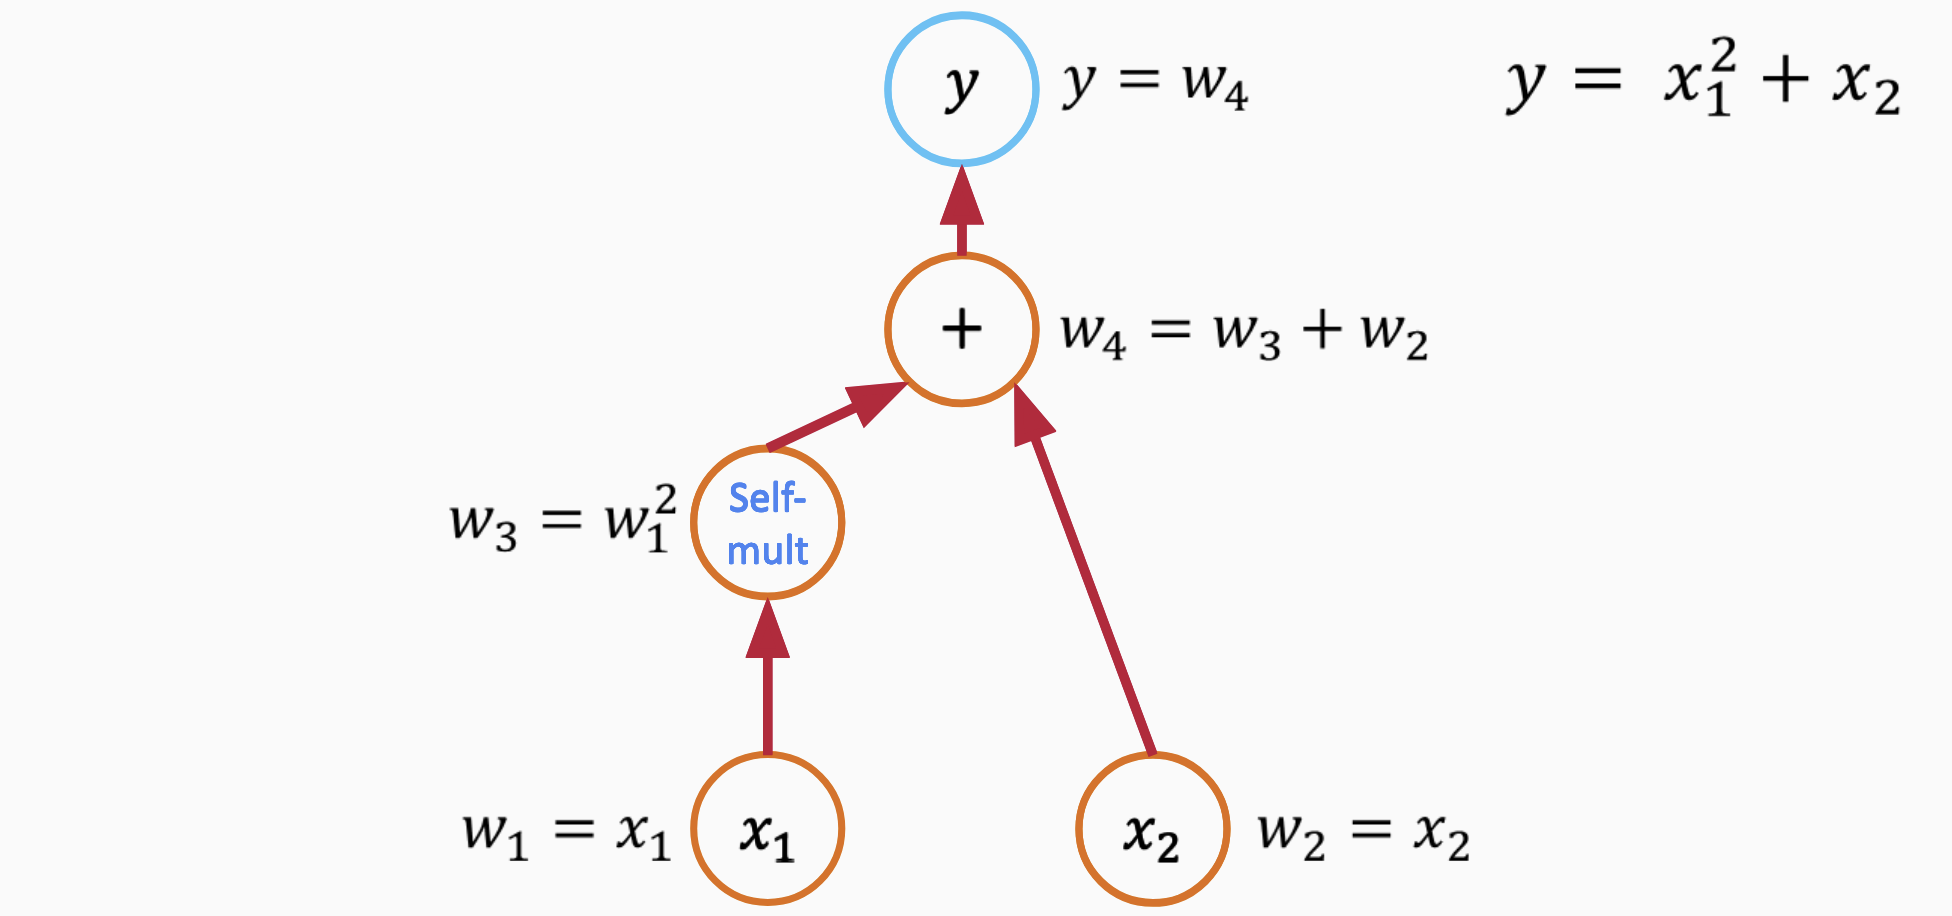
\includegraphics[width=0.8\textwidth]{figs/ad2.png}
\end{figure}

\end{frame}

%------------------------------------------------
\begin{frame}
\frametitle{Decomposition into Elementary Steps}

We can break down the graph and assign intermediate variables.

\begin{columns}[T]
    \begin{column}{0.4\textwidth}
        \textbf{Evaluation Trace:}
        \begin{enumerate}
            \item $v_1 = x_1^2$
            \item $y = v_1 + x_2$
        \end{enumerate}
        
        \vspace{1cm}
        
        This decomposition is the key that makes AD possible. By applying the chain rule to each elementary step, we can compute exact derivatives.
        
    \end{column}
    \begin{column}{0.6\textwidth}
        \begin{figure}[ht]
        	\centering
        	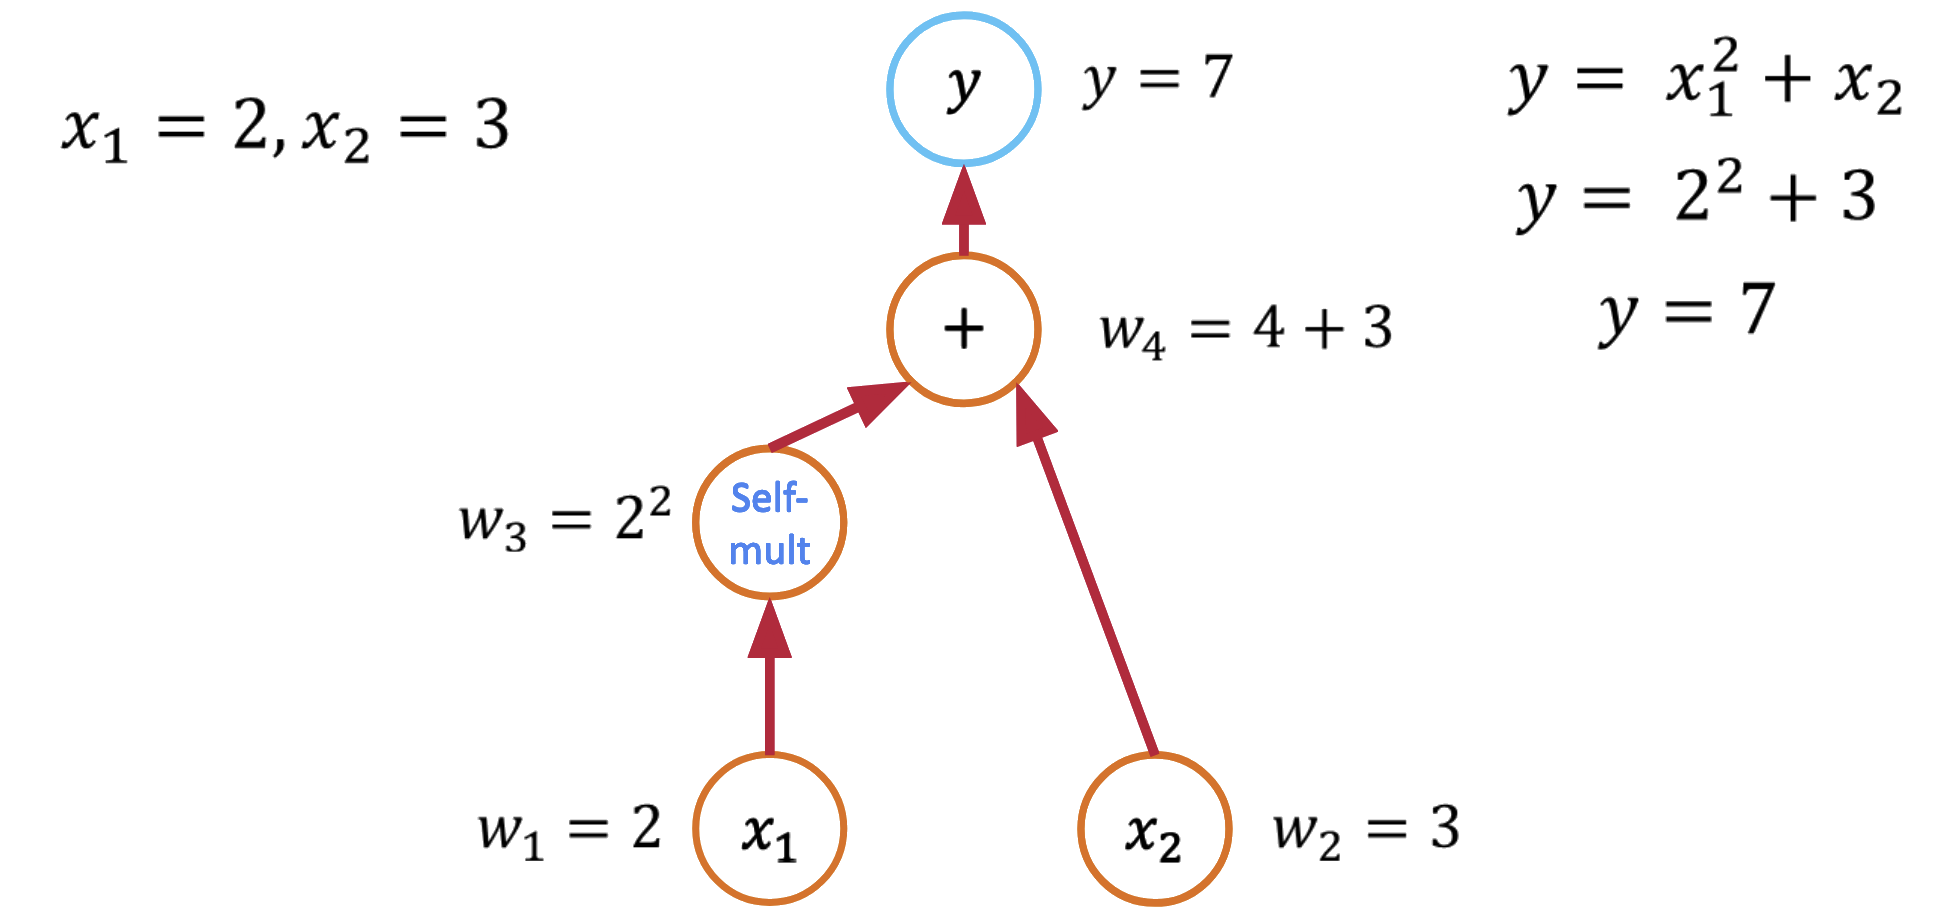
\includegraphics[width=\linewidth]{figs/ad3.png}
        \end{figure}
    \end{column}
\end{columns}


\end{frame}

%----------------------------------------------------------------------------------------
\section{Forward Mode AD}
%----------------------------------------------------------------------------------------

\begin{frame}
\frametitle{Forward Mode Automatic Differentiation}

Forward mode AD propagates derivative information \textbf{forward} through the graph, alongside the function evaluation.

\begin{figure}[ht]
	\centering
	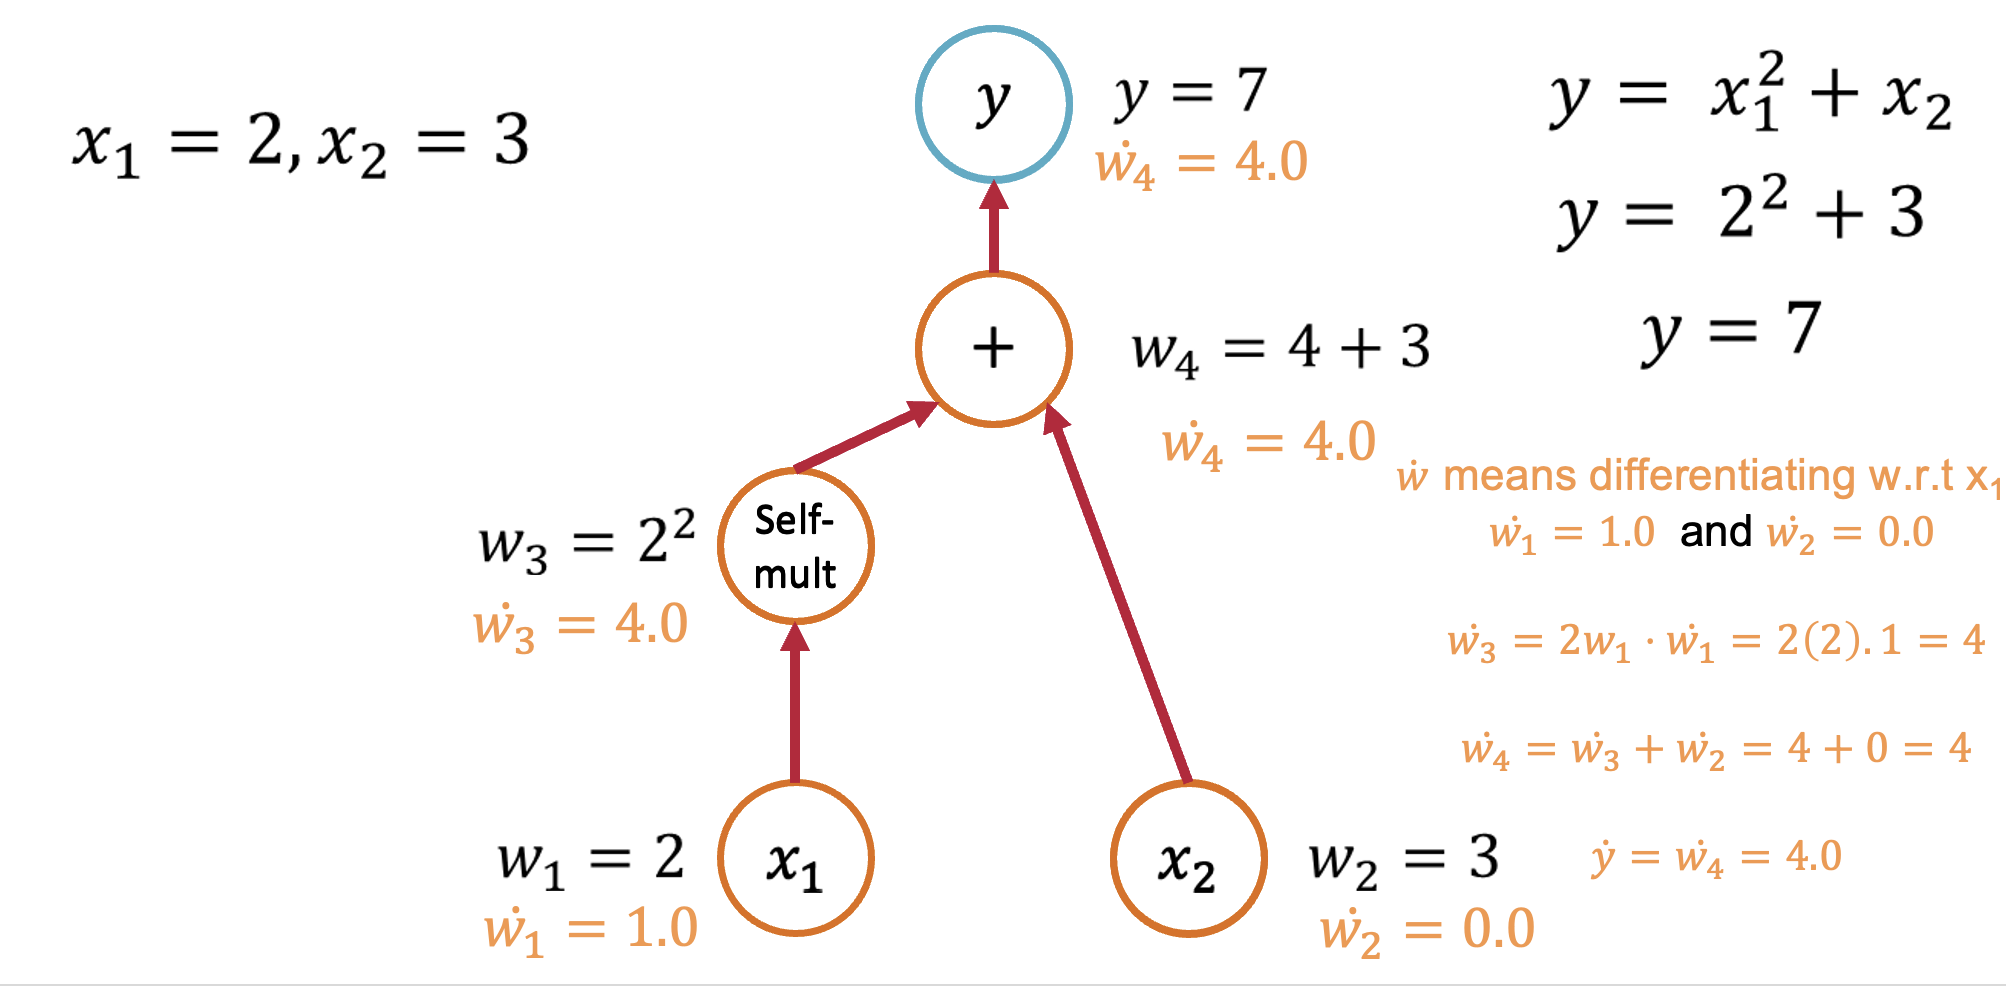
\includegraphics[width=\textwidth]{figs/forward-mode-ad.png}
\end{figure}

\end{frame}

%------------------------------------------------
\begin{frame}
\frametitle{Forward Mode: Step-by-Step Example}

Let's compute $\frac{\partial y}{\partial x_1}$ for $y = x_1^2 + x_2$.

\begin{block}{1. Seed the input w.r.t. $x_1$}
Set $\dot{x}_1 = 1$ and $\dot{x}_2 = 0$.
\end{block}

\begin{block}{2. Forward Propagation}
\begin{itemize}
    \item $v_1 = x_1^2 \implies \dot{v}_1 = 2x_1 \cdot \dot{x}_1 = 2x_1 \cdot 1 = 2x_1$
    \item $y = v_1 + x_2 \implies \dot{y} = \dot{v}_1 + \dot{x}_2 = 2x_1 + 0 = 2x_1$
\end{itemize}
\end{block}

\begin{alertblock}{Result}
The final propagated tangent $\dot{y}$ is the derivative: $\frac{\partial y}{\partial x_1} = 2x_1$.
\end{alertblock}

\textbf{Key Idea:} To get the derivative w.r.t. $x_2$, we would need a \textit{new pass} with seeds $\dot{x}_1 = 0, \dot{x}_2 = 1$.

\end{frame}

%----------------------------------------------------------------------------------------
\section{Reverse Mode AD (Backpropagation)}
%----------------------------------------------------------------------------------------

\begin{frame}
\frametitle{Reverse Mode Automatic Differentiation}

Reverse mode AD (or \textbf{backpropagation}) computes derivatives by propagating information \textbf{backward} from the output.

\textbf{Algorithm:}
\begin{enumerate}
    \item \textbf{Forward Pass:} Evaluate the function and store all intermediate values.
    \item \textbf{Backward Pass:} Starting from the output, use the chain rule to propagate "adjoints" ($\bar{v} = \frac{\partial y}{\partial v}$) backward through the graph.
\end{enumerate}

\end{frame}

\begin{frame}
	\frametitle{Reverse Mode Automatic Differentiation}
	
	Reverse mode AD (or \textbf{backpropagation}) computes derivatives by propagating information \textbf{backward} from the output.
	
	\begin{figure}[ht]
		\centering
		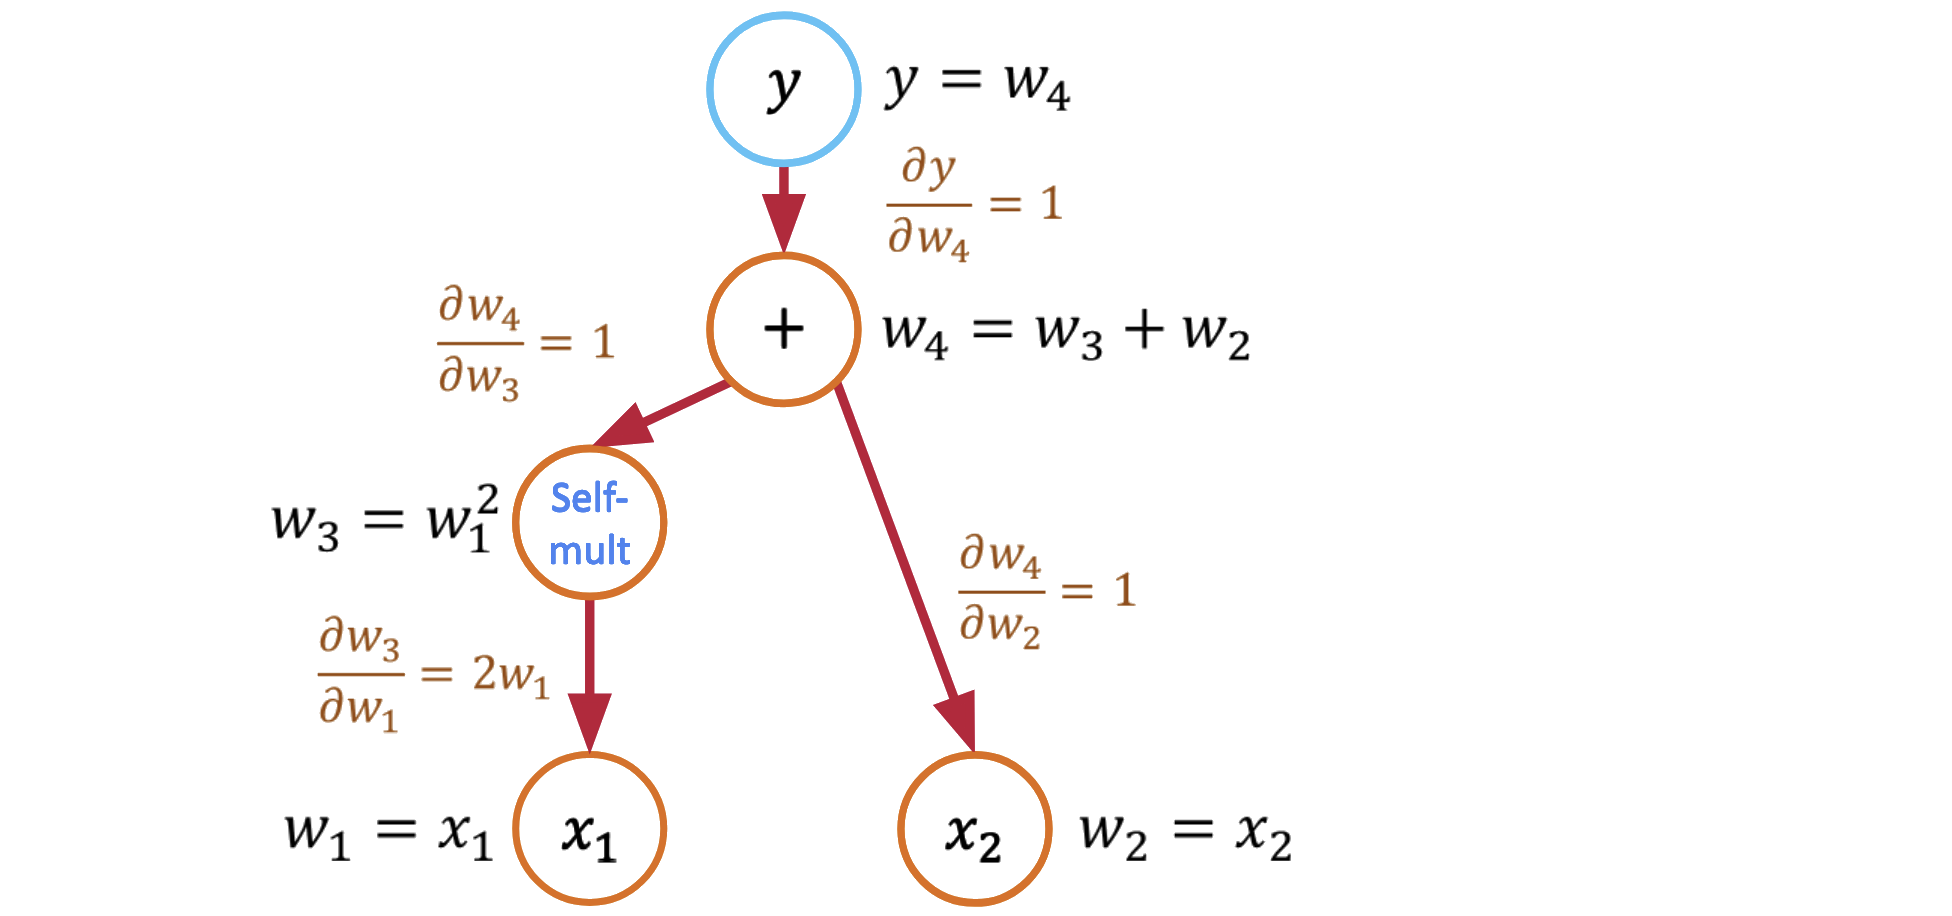
\includegraphics[width=0.9\textwidth]{figs/ad4.png}
	\end{figure}
	
\end{frame}

%----------------------------------------------
\begin{frame}
	\frametitle{Reverse Mode: The Power of the Chain Rule}
	
	The backward pass systematically applies the chain rule.
	
	Let's trace the computation for $y = x_1^2 + x_2$:
	
	\begin{figure}[ht]
		\centering
		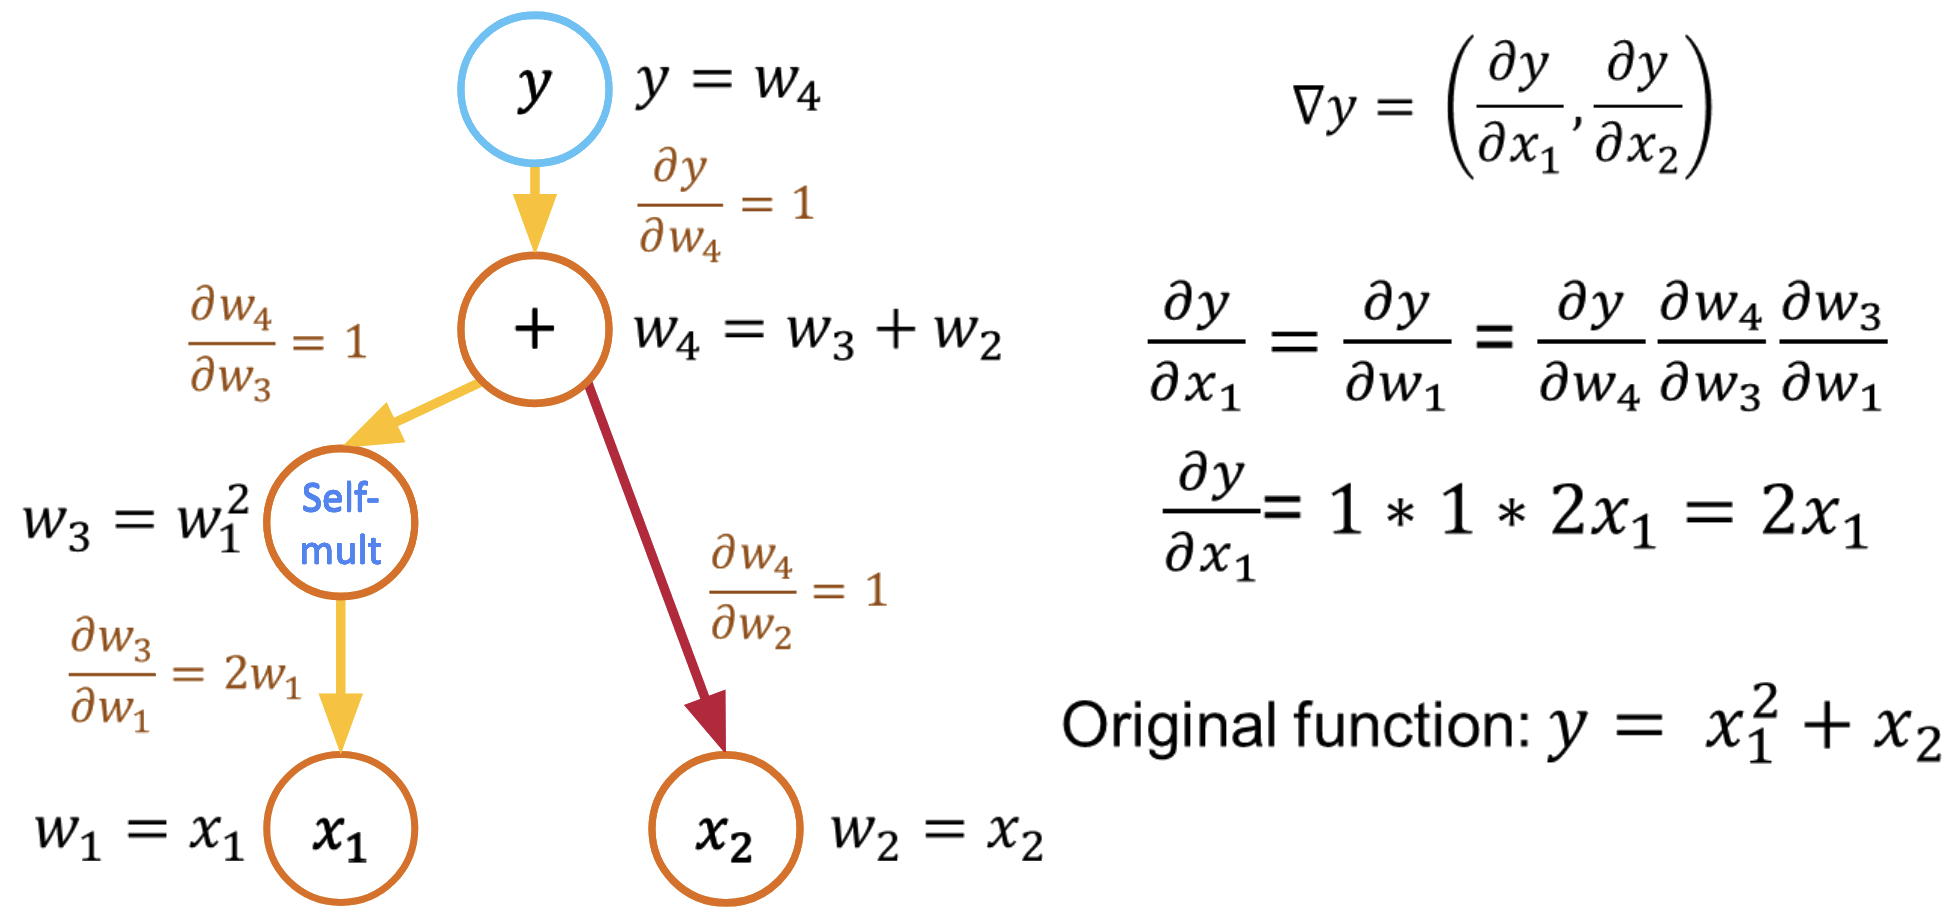
\includegraphics[width=\textwidth]{figs/ad6.png}
	\end{figure}
	
\end{frame}


%------------------------------------------------
\begin{frame}
\frametitle{Reverse Mode: One Pass for All Gradients}

The magic of reverse mode: it computes \textbf{all} partial derivatives in a single backward pass.

\begin{block}{1. Forward Pass \& Seed Output}
Evaluate $y = x_1^2 + x_2$ and set $\bar{y} = \frac{\partial y}{\partial y} = 1$.
\end{block}

\begin{block}{2. Backward Pass}
\begin{itemize}
    \item $\bar{v}_1 = \bar{y} \cdot \frac{\partial y}{\partial v_1} = 1 \cdot 1 = 1$
    \item $\bar{x}_2 = \bar{y} \cdot \frac{\partial y}{\partial x_2} = 1 \cdot 1 = 1 \implies \frac{\partial y}{\partial x_2} = 1$
    \item $\bar{x}_1 = \bar{v}_1 \cdot \frac{\partial v_1}{\partial x_1} = 1 \cdot 2x_1 = 2x_1 \implies \frac{\partial y}{\partial x_1} = 2x_1$
\end{itemize}
\end{block}

\end{frame}

%------------------------------------------------
\begin{frame}
	\frametitle{Reverse Mode: One Pass for All Gradients}
	\begin{figure}[ht]
		\centering
		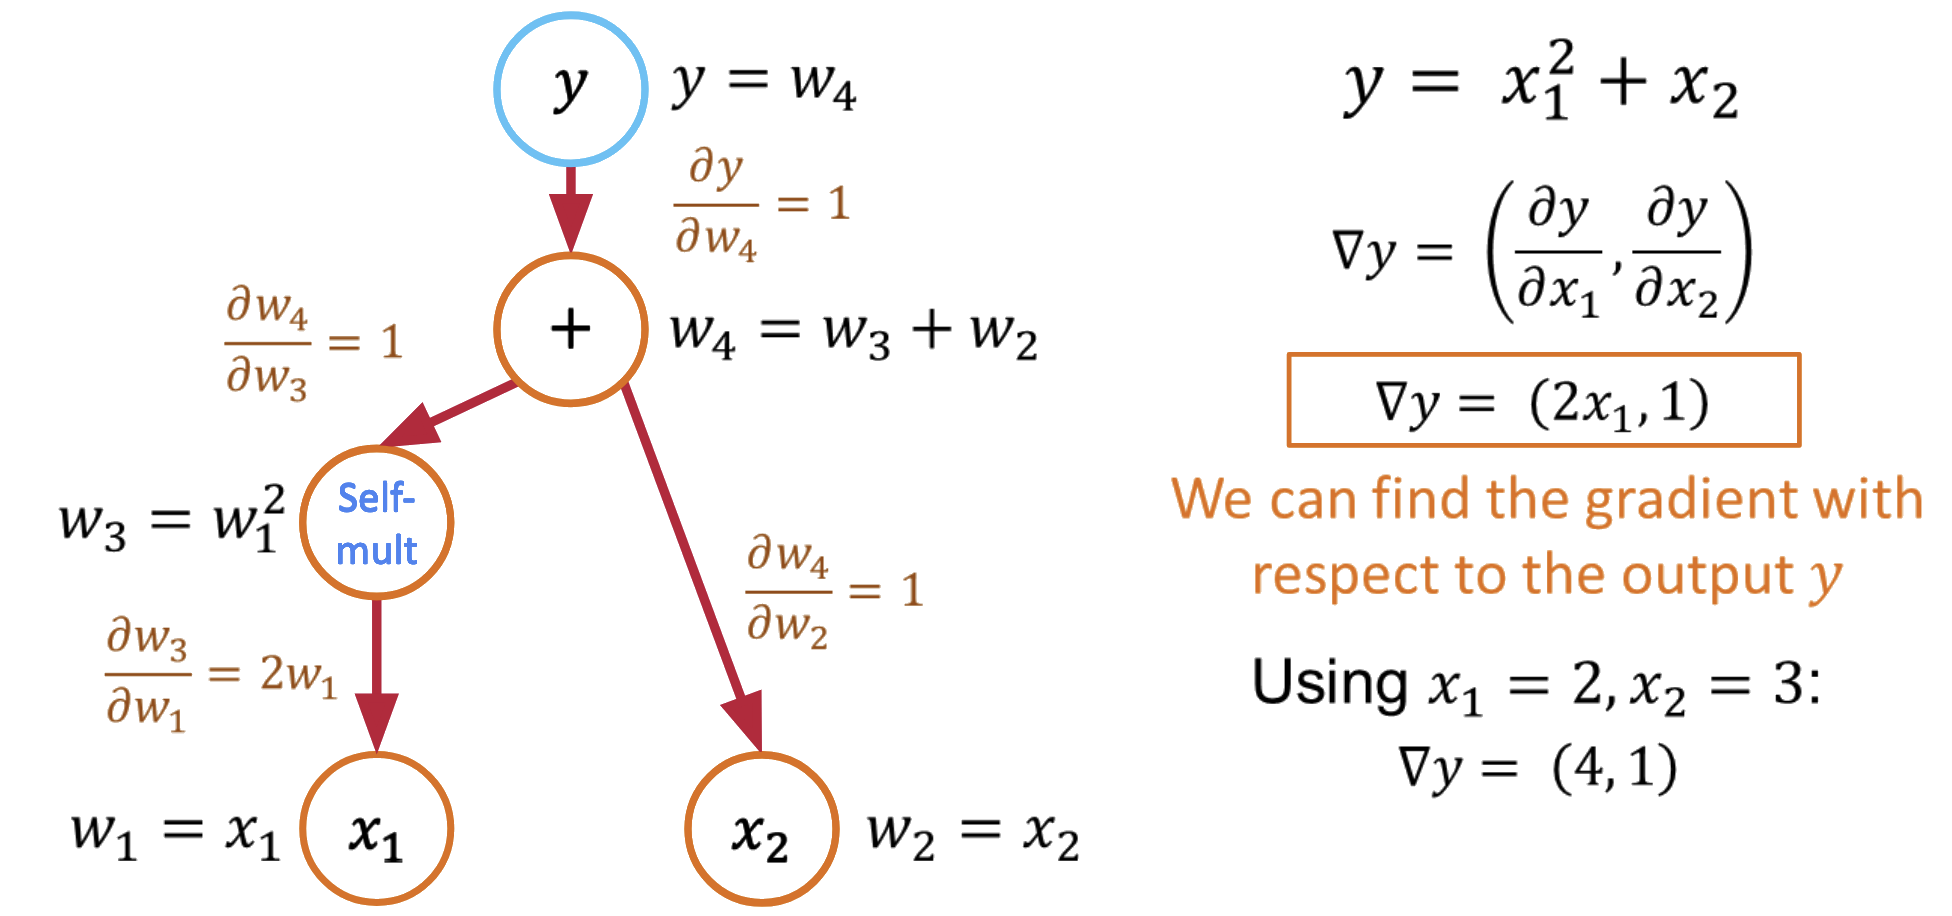
\includegraphics[width=\textwidth]{figs/ad7.png}
	\end{figure}
	
\end{frame}

%----------------------------------------------------------------------------------------
\section{Forward vs. Reverse Mode}
%----------------------------------------------------------------------------------------

\begin{frame}
\frametitle{When to Use Forward vs. Reverse Mode}

The choice depends on the dimensions of your function $f: \mathbb{R}^n \to \mathbb{R}^m$.

\begin{columns}[T]
    \begin{column}{0.48\textwidth}
        \begin{block}{Forward Mode}
        \begin{itemize}
            \item \textbf{Cost:} One pass per \textit{input} variable.
            \item \textbf{Efficient when:} Few inputs, many outputs ($n \ll m$).
            \item \textbf{Computes:} Jacobian-vector products ($J \cdot v$).
        \end{itemize}
        \end{block}
    \end{column}
    \hfill
    \begin{column}{0.48\textwidth}
        \begin{block}{Reverse Mode}
        \begin{itemize}
            \item \textbf{Cost:} One pass per \textit{output} variable.
            \item \textbf{Efficient when:} Many inputs, few outputs ($n \gg m$).
            \item \textbf{Computes:} Vector-Jacobian products ($v^T \cdot J$).
        \end{itemize}
        \end{block}
    \end{column}
\end{columns}

\vspace{1cm}

\textbf{Machine Learning context:} We have millions of parameters (inputs, $n$) and a single scalar loss function (output, $m=1$).
\begin{center}
\textbf{Reverse mode is the clear winner!}
\end{center}

\end{frame}

%----------------------------------------------------------------------------------------
\section{AD in Practice: PyTorch}
%----------------------------------------------------------------------------------------

\begin{frame}[fragile]
\frametitle{AD in PyTorch: A Simple Example}

PyTorch's `autograd` engine is built on reverse-mode AD.

\begin{lstlisting}[style=pythonstyle]
import torch

# Define variables that require gradients
x1 = torch.tensor(2.0, requires_grad=True)
x2 = torch.tensor(3.0, requires_grad=True)

# Define the function
y = x1**2 + x2

# Compute gradients using reverse mode AD
y.backward()

# Access the computed gradients
# dy/dx1 = 2*x1 = 4.0
print(f"dy/dx1: {x1.grad.item()}")
# dy/dx2 = 1.0
print(f"dy/dx2: {x2.grad.item()}")
\end{lstlisting}

\begin{block}{Output}
\begin{verbatim}
dy/dx1: 4.0
dy/dx2: 1.0
\end{verbatim}
\end{block}

\end{frame}

%------------------------------------------------
\begin{frame}[fragile]
\frametitle{AD in PyTorch: Neural Network}

The power of AD becomes clear with complex models. PyTorch automatically computes gradients for all network parameters.

\begin{lstlisting}[style=pythonstyle]
import torch.nn as nn

net = SimpleNet() # 2-layer NN
x = torch.tensor([[1.0, 2.0]])
target = torch.tensor([[0.5]])

# Forward pass
output = net(x)
loss = ((output - target)**2).mean()

# Backward pass - computes gradients for ALL parameters
loss.backward()

# Access gradients
for name, param in net.named_parameters():
    print(f"{name}: grad shape {param.grad.shape}")
\end{lstlisting}

\begin{block}{Output}
\begin{verbatim}
layer1.weight: gradient shape torch.Size([3, 2])
layer1.bias: gradient shape torch.Size([3])
layer2.weight: gradient shape torch.Size([1, 3])
layer2.bias: gradient shape torch.Size([1])
\end{verbatim}
\end{block}

\end{frame}

%-------------------------------------------------------------------

\begin{frame}
\frametitle{The AD Revolution}

Automatic differentiation has revolutionized scientific computing by making gradients:

\begin{enumerate}
    \item \textbf{Ubiquitous:} Available for any differentiable code.
    \item \textbf{Exact:} No approximation errors (up to machine precision).
    \item \textbf{Efficient:} Cost is proportional to the original function evaluation.
    \item \textbf{Automatic:} No tedious and error-prone manual derivation required.
\end{enumerate}

\vspace{0.5cm}

This has enabled the deep learning revolution and is now reshaping scientific discovery through differentiable programming.

\end{frame}

%------------------------------------------------
\begin{frame}
\frametitle{Looking Forward}

AD is the mathematical engine powering the new era of Scientific Machine Learning:

\begin{itemize}
    \item Physics-Informed Neural Networks (PINNs)
    \item Neural Differential Equations
    \item Differentiable Simulators
    \item End-to-end optimization of entire scientific workflows
\end{itemize}

\vspace{1cm}

The ability to compute gradients automatically through arbitrary code is a fundamental capability that is reshaping how we approach science in the 21st century.

\end{frame}

%------------------------------------------------
\begin{frame}
\frametitle{Questions?}

\centering
\Large Thank you!

\vspace{2cm}

\textbf{Contact:} \\
Krishna Kumar \\
\textit{krishnak@utexas.edu} \\
University of Texas at Austin

\end{frame}

\end{document}